\chapter{ یادگیری تقویتی}
\section{مقدمه}
به طور عمومی، یادگیری ماشین به دسته‌ای از الگوریتم‌ها و روش‌های محاسباتی گفته می‌شود که به ماشین‌ها امکان یادگیری از داده‌ها و تجربه‌های خود را می‌دهند.
یادگیری ماشین به دو دسته‌ی اصلی تقسیم می‌شود: یادگیری نظارت‌شده و یادگیری بدون نظارت.
در یادگیری نظارت‌شده، مدل به کمک داده‌های برچسب‌خورده آموزش داده می‌شود، و سپس برای پیش‌بینی خروجی‌های جدید از این مدل استفاده می‌شود.
در یادگیری بدون نظارت، مدل بدون داده‌های برچسب‌خورده آموزش داده می‌شود، و باید خودش مفاهیم و الگوهای موجود در داده‌ها را کشف کند.
یادگیری تقویتی در این دو دسته قرار نمی‌گیرد، و به عنوان یک دسته جداگانه در نظر گرفته می‌شود.

یادگیری تقویتی یک روش یادگیری ماشین است که به عامل اجازه می‌دهد تا رفتار بهینه را از طریق تعامل و آزمون و خطا با محیط یاد بگیرد.
در این روش، عامل مشاهدات خود را از محیط (به کمک سنسور)
دریافت کرده،
و بر اساس آن تصمیم خود را اخذ می‌کند.
پس از انجام هر عمل، محیط به عامل پاداشی می‌دهد که نشان‌دهنده‌ی عملکرد عامل در آن حالت است.
هدف این است که عامل مجموع پاداش‌های دریافتی خود را بیشینه کند، که در صورت صحیح بودن تعریف سیگنال پاداش، معمولا به معنای رسیدن به هدف مطلوب است.

یادگیری ماشین با سایر رویکرد‌های یادگیری ماشین مانند یادگیری نظارت‌شده و یادگیری بدون نظارت تفاوت‌های زیادی دارد، 
و معمولا بر مسائلی به کار می‌رود که تمرکز بر تصمیم‌گیری یا پیدا کردن سیاست بهینه بدون نیاز به داده‌های برچسب‌خورده است.
در عوض، عامل با اکتشاف و بهره‌برداری ابتدا انتقالات بین حالت‌ها و پاداش‌های مرتبط با آن‌ها را یاد می‌گیرد، و سپس سیاستی را یاد می‌گیرد که مجموع پاداش‌ها را بیشینه کند.


\section{اصول یادگیری تقویتی}
\subsection{عامل، محیط، حالت، عمل و پاداش}
در یادگیری تقویتی، عامل \LTRfootnote{Agent}
 تصمیم‌گیرنده برای رسیدن به هدف خود با محیط\LTRfootnote{Environment}
  تعامل دارد.
محیط معمولا به صورت مجموعه‌ای از حالت‌ها \LTRfootnote{State}
  و عمل‌هایی \LTRfootnote{Action}
    که عامل می‌تواند انجام دهد مدل می‌شود.
در هر گام، عامل مشاهده‌ای از حالت محیط را دریافت می‌کند و بر اساس آن تصمیمی اتخاذ می‌کند.
پس از انجام عمل، محیط به عامل پاداش \LTRfootnote{Reward}
  می‌دهد که نشان‌دهنده‌ی عملکرد عامل در آن حالت است.

\begin{figure}[H]
    \centering
    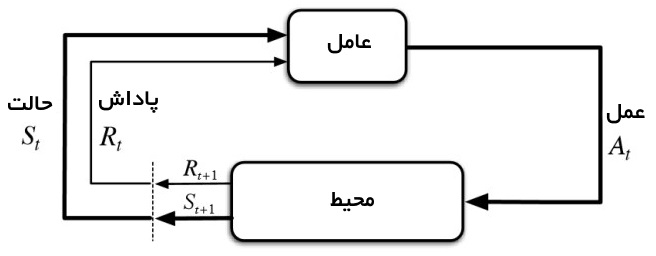
\includegraphics[width=0.75\textwidth]{images/agent_env.jpg}
    \caption{تعامل عامل و محیط}\label{fig:agent_env}

\end{figure}
% explain episodes here
در اکثر مواقع، یادگیری تقویتی در مسائلی استفاده می‌شود، که بتوان آن را به دنباله‌ای از گام‌ها تقسیم کرد که قطعا به یک حالت پایانی می‌رسد.
 هر یک از این دنباله‌ها را قسمت \LTRfootnote{Episode}
  می‌نامند.
\subsection{فرایند تصمیم‌گیری مارکوف}
فرایند تصمیم‌گیری مارکوف \LTRfootnote{Markov Decision Process (MDP)}
  مدلی است برای تصمیم‌گیری در محیط‌هایی که به صورت مارکوف هستند.
  محیط‌های دارای خاصیت مارکوف، محیط‌هایی هستند که حالت بعدی به صورت کامل به حالت فعلی و عمل انجام شده وابسته است.


  یک فرایند تصمیم‌گیری مارکوف، چهارتایی 
  $(S, A, P, R)$
  است که در آن:
  \begin{itemize}
      \item $S$ مجموعه‌ی تمام حالت‌های ممکن محیط است.
      \item $A$ مجموعه‌ی تمام عمل‌های ممکن است.
      \item $P$ تابع انتقال \LTRfootnote{Transition Function}
      است که به ازای هر حالت و عمل، توزیع احتمال حالت بعدی را مشخص می‌کند.
      \item $R$ تابع پاداش \LTRfootnote{Reward Function}
      است که به ازای هر حالت و عمل، پاداش مورد انتظار را مشخص می‌کند.
      \item فاکتور تخفیف $\gamma$ نیز معمولا به عنوان یک پارامتر دیگر در نظر گرفته می‌شود که نشان‌دهنده‌ی اهمیت پاداش‌های آینده نسبت به پاداش‌های فعلی است.
  \end{itemize}
همانطور که گفته شد، در هر گام عامل با اخذ تصمیم خود، محیط را به حالت جدیدی می‌برد و پاداشی دریافت می‌کند.
به مجموع کل پاداش‌هایی که عامل در یک قسمت دریافت می‌کند، خروجی \LTRfootnote{Return}
 گفته می‌شود.
 \begin{equation}\label{eq:return}
     G_t = R_{t+1} + \gamma \times R_{t+2} + \gamma^2 \times R_{t+3} + \cdots = \sum_{k=0}^\infty \gamma^k \times R_{t+k+1}
 \end{equation}
\subsection{سیاست، تابع ارزش، و تابع ارزش عمل}
سیاست \LTRfootnote{Policy}
یک تابع از حالت‌ها به عمل‌ها است که نشان‌دهنده‌ی رفتار عامل در هر حالت محیط است.
در واقع مسئله یادگیری تقویتی را می‌توان به ((یافتن سیاستی که مجموع پاداش‌ها را بیشینه می‌کند)) تعبیر کرد.
\begin{equation}\label{eq:policy}
    \pi(a|s) = \mathbb{P}\{A_t = a | S_t = s\}
\end{equation}

تابع ارزش \LTRfootnote{Value Function} $V(s)$
یک تابع از حالت‌ها است که نشان‌دهنده‌ی میزان پاداش مورد انتظار از یک حالت تا به انتهای قسمت است.
\begin{equation}\label{eq:value_function}
    v_\pi(s) = \mathbb{E}_\pi\{G_t | S_t = s\} = \sum_{a \in A}\pi(a|s)\times\{R_s^a + \gamma \times \sum_{s' \in S}p(s'|s,a)\times v_\pi(s')\}
\end{equation}
تابع ارزش عمل \LTRfootnote{Action Value Function} $Q(s, a)$
نیز مشابه تابع ارزش است، با این تفاوت که به جای حالت، از یک حالت و یک عمل مشخص محاسبه می‌شود. رایج است که به این تابع، تابع کیو گفته شود.
\begin{equation}\label{eq:q_function}
    q_\pi(s,a) = \mathbb{E}_\pi\{G_t | S_t = s, A_t = a\} = R_s^a + \gamma \times \sum_{s' \in S}p(s'|s,a)\times v_\pi(s')
\end{equation}
به این معادلات، که از کلیدی‌ترین روابط در یادگیری تقویتی هستند، معادله بلمن \LTRfootnote{Bellman Equation} گفته می‌شود.
\section{الگوریتم‌های پایه یادگیری تقویتی}
\subsection{برنامه‌نویسی پویا}
همان‌طور که در معادله \ref{eq:value_function} مشخص است، می‌توان تابع ارزش را به صورت بازگشتی محاسبه کرد.
این روش برنامه‌نویسی پویا \LTRfootnote{Dynamic Programming}
نام دارد.
\subsubsection{یادگیری به کمک تکرار ارزش}
در روش تکرار ارزش \LTRfootnote{Value Iteration}،
، ابتدا تابع ارزش را به صورت تصادفی مقداردهی می‌کنیم و سپس آن را به صورت بازگشتی به روزرسانی می‌کنیم.
قابل اثبات است که این روش به تابع ارزش بهینه همگرا می‌شود.
به صورت شهودی نیز، می‌توان دید که ارزش از سمت حالت‌های پایانی به سمت حالت‌های ابتدایی به روزرسانی می‌شود.
\subsubsection{یادگیری به کمک تکرار سیاست}
در روش تکرار سیاست \LTRfootnote{Policy Iteration}،
ابتدا سیاست را به صورت تصادفی مقداردهی می‌کنیم و سپس تابع ارزش را برای آن محاسبه می‌کنیم.
سپس سیاست را به صورت بازگشتی به روزرسانی می‌کنیم. 
این فرآیند را تا زمانی که سیاست تغییر نکند ادامه می‌دهیم.
قابل اثبات است که این روش به سیاست بهینه همگرا می‌شود.

در عمل، با توجه به اینکه معمولا به تابع انتقال دسترسی نداریم، نمی‌توانیم از روش‌های برنامه‌نویسی پویا به صورت مستقیم استفاده کنیم.
در واقع نیاز به راه حل‌های مستقل از مدل داریم که به کمک نمونه‌برداری و کاوش محیط، سیاست بهینه را یاد بگیرند.

\subsection{یادگیری به کمک نمونه‌برداری مونته کارلو}
در روش‌های یادگیری به کمک نمونه‌برداری مونته کارلو \LTRfootnote{Monte Carlo Sampling}،
به جای استفاده از مدل، از نمونه‌برداری برای تخمین ارزش استفاده می‌شود.
کافی‌ست ابتدا یک قسمت را به طور کامل اجرا کنیم، و سپس ارزش هر حالت را، به سمت خروجی قسمت، به روزرسانی کنیم:
\begin{equation}\label{eq:mc_q_function}
    Q(s_t, a_t) = Q(s_t, a_t) + \alpha \times (G_t - Q(s_t, a_t))
\end{equation}
که در این فرمول، $\alpha$
نرخ یادگیری \LTRfootnote{Learning Rate} است.

لازم به ذکر است که در حین اجرای قسمت، از سیاست اپسیلون-حریصانه \LTRfootnote{$\epsilon$-greedy} استفاده می‌شود.
در این سیاست، با احتمال $\epsilon$ عملی تصادفی انجام می‌شود و با احتمال $1-\epsilon$ عملی که ارزش بیشتری دارد انجام می‌شود.
دلیل استفاده از این سیاست، نیاز به کاوش محیط و جلوگیری از گیر کردن در حالت‌های محلی است.

از معایب این روش، می‌توان به نیاز به اجرای کامل قسمت‌ها و نیاز به زمان برای یادگیری اشاره کرد. به همین دلیل، این روش برای مسائلی که قسمت‌های طولانی دارند، مناسب نیست.
از مشکلات دیگر این روش، عدم استفاده از ویژگی مارکوف محیط است.
\subsection{یادگیری به کمک تفاوت زمانی}
همان‌طور که گفته شد، استفاده از یادگیری مونته‌کارلو باعث می‌شود که عامل در حین انجام قسمت، از تجربه‌ی قبلی خود استفاده نکند
و به روز رسانی ارزش‌ها فقط پس از اتمام قسمت انجام شود. به این روش، یادگیری آفلاین \LTRfootnote{Offline Learning} گفته می‌شود.
در روش یادگیری به کمک تفاوت زمانی \LTRfootnote{Temporal Difference Learning}،
عامل در حین انجام قسمت، از تجربه‌ی خود استفاده می‌کند و ارزش‌ها را به صورت آنلاین به روزرسانی می‌کند.
در واقع به کمک معادله بلمن، مقادیر کیو به سمت مقدار کیو بعدی به روزرسانی می‌شوند.

پیاده‌سازی این دو الگوریتم، به دو روش دید رو به جلو و دید رو به عقب انجام می‌شود.
در حالت دید رو به جلو، مشابه با یادگیری مونته کارلو، پس از رسیدن به پایان قسمت، ارزش‌ها به روزرسانی می‌شوند.
در حالت دید رو به عقب، ارزش‌ها به صورت آنلاین به روزرسانی می‌شوند. به این صورت که پس از دریافت یک پاداش، عامل مقادیر کیو $n$ حالت‌ قبلی خود را به روزرسانی می‌کند.
\subsubsection{تی‌دی صفر}
در ساده‌ترین حالت، عامل در حین انجام عمل، با دیدن یک گام در آینده یا گذشته، ارزش عمل فعلی را به روزرسانی می‌کند.
به این روش تی‌دی صفر \LTRfootnote{TD(0)} گفته می‌شود.
\begin{equation}\label{eq:td_zero_q_function}
    Q(s_t, a_t) = Q(s_t, a_t) + \alpha \times (R_{t+1} + \gamma \times Q(s_{t+1}, a_{t+1}) - Q(s_t, a_t))
\end{equation}
در واقع، به کمک رابطه بلمن
(که فرم ارزش عمل آن در رابطه  \ref{eq:q_function} دیده می‌شود)
میزان صحیح بودن ارزش عمل فعلی، با ارزش عمل بعدی و پاداش فعلی مقایسه می‌شود و ارزش عمل فعلی به روزرسانی می‌شود.
\subsubsection{ تی‌دی لامبدا رو به جلو}
در روش تی‌دی $\lambda$،
\LTRfootnote{TD($\lambda$)}
با دید رو به جلو
به جای استفاده از یک گام در آینده ، از یک ترکیب خطی از پاداش‌ها و بازگشت چندین گام استفاده می‌شود.
به این ترکیب خطی، $\lambda$-بازگشت \LTRfootnote{$\lambda$-return} گفته می‌شود.
\begin{equation}\label{eq:td_lambda_q_function}
    Q(s_t, a_t) = Q(s_t, a_t) + \alpha \times (G_t^\lambda - Q(s_t, a_t))
\end{equation}
که در این رابطه، $G_t^\lambda$
به صورت زیر محاسبه می‌شود:
\begin{equation}\label{eq:td_lambda_return}
    G_t^\lambda = (1-\lambda)\times\sum_{n=1}^\infty \lambda^{n-1} \times G_t^{(n)}
\end{equation}
که در آن $G_t^{(n)}$، 
مقدار بازگشتی بعد از $n$ گام است،
و $\lambda$
یک پارامتر بین صفر و یک است که نشان‌دهنده‌ی اهمیت پاداش‌های آینده نسبت به پاداش‌های فعلی است.
می‌توان میزان اهمیت پاداش‌های را به ازای مقادیر مختلف $\lambda$ مشاهده کرد.
\begin{figure}[H]
    \centering
    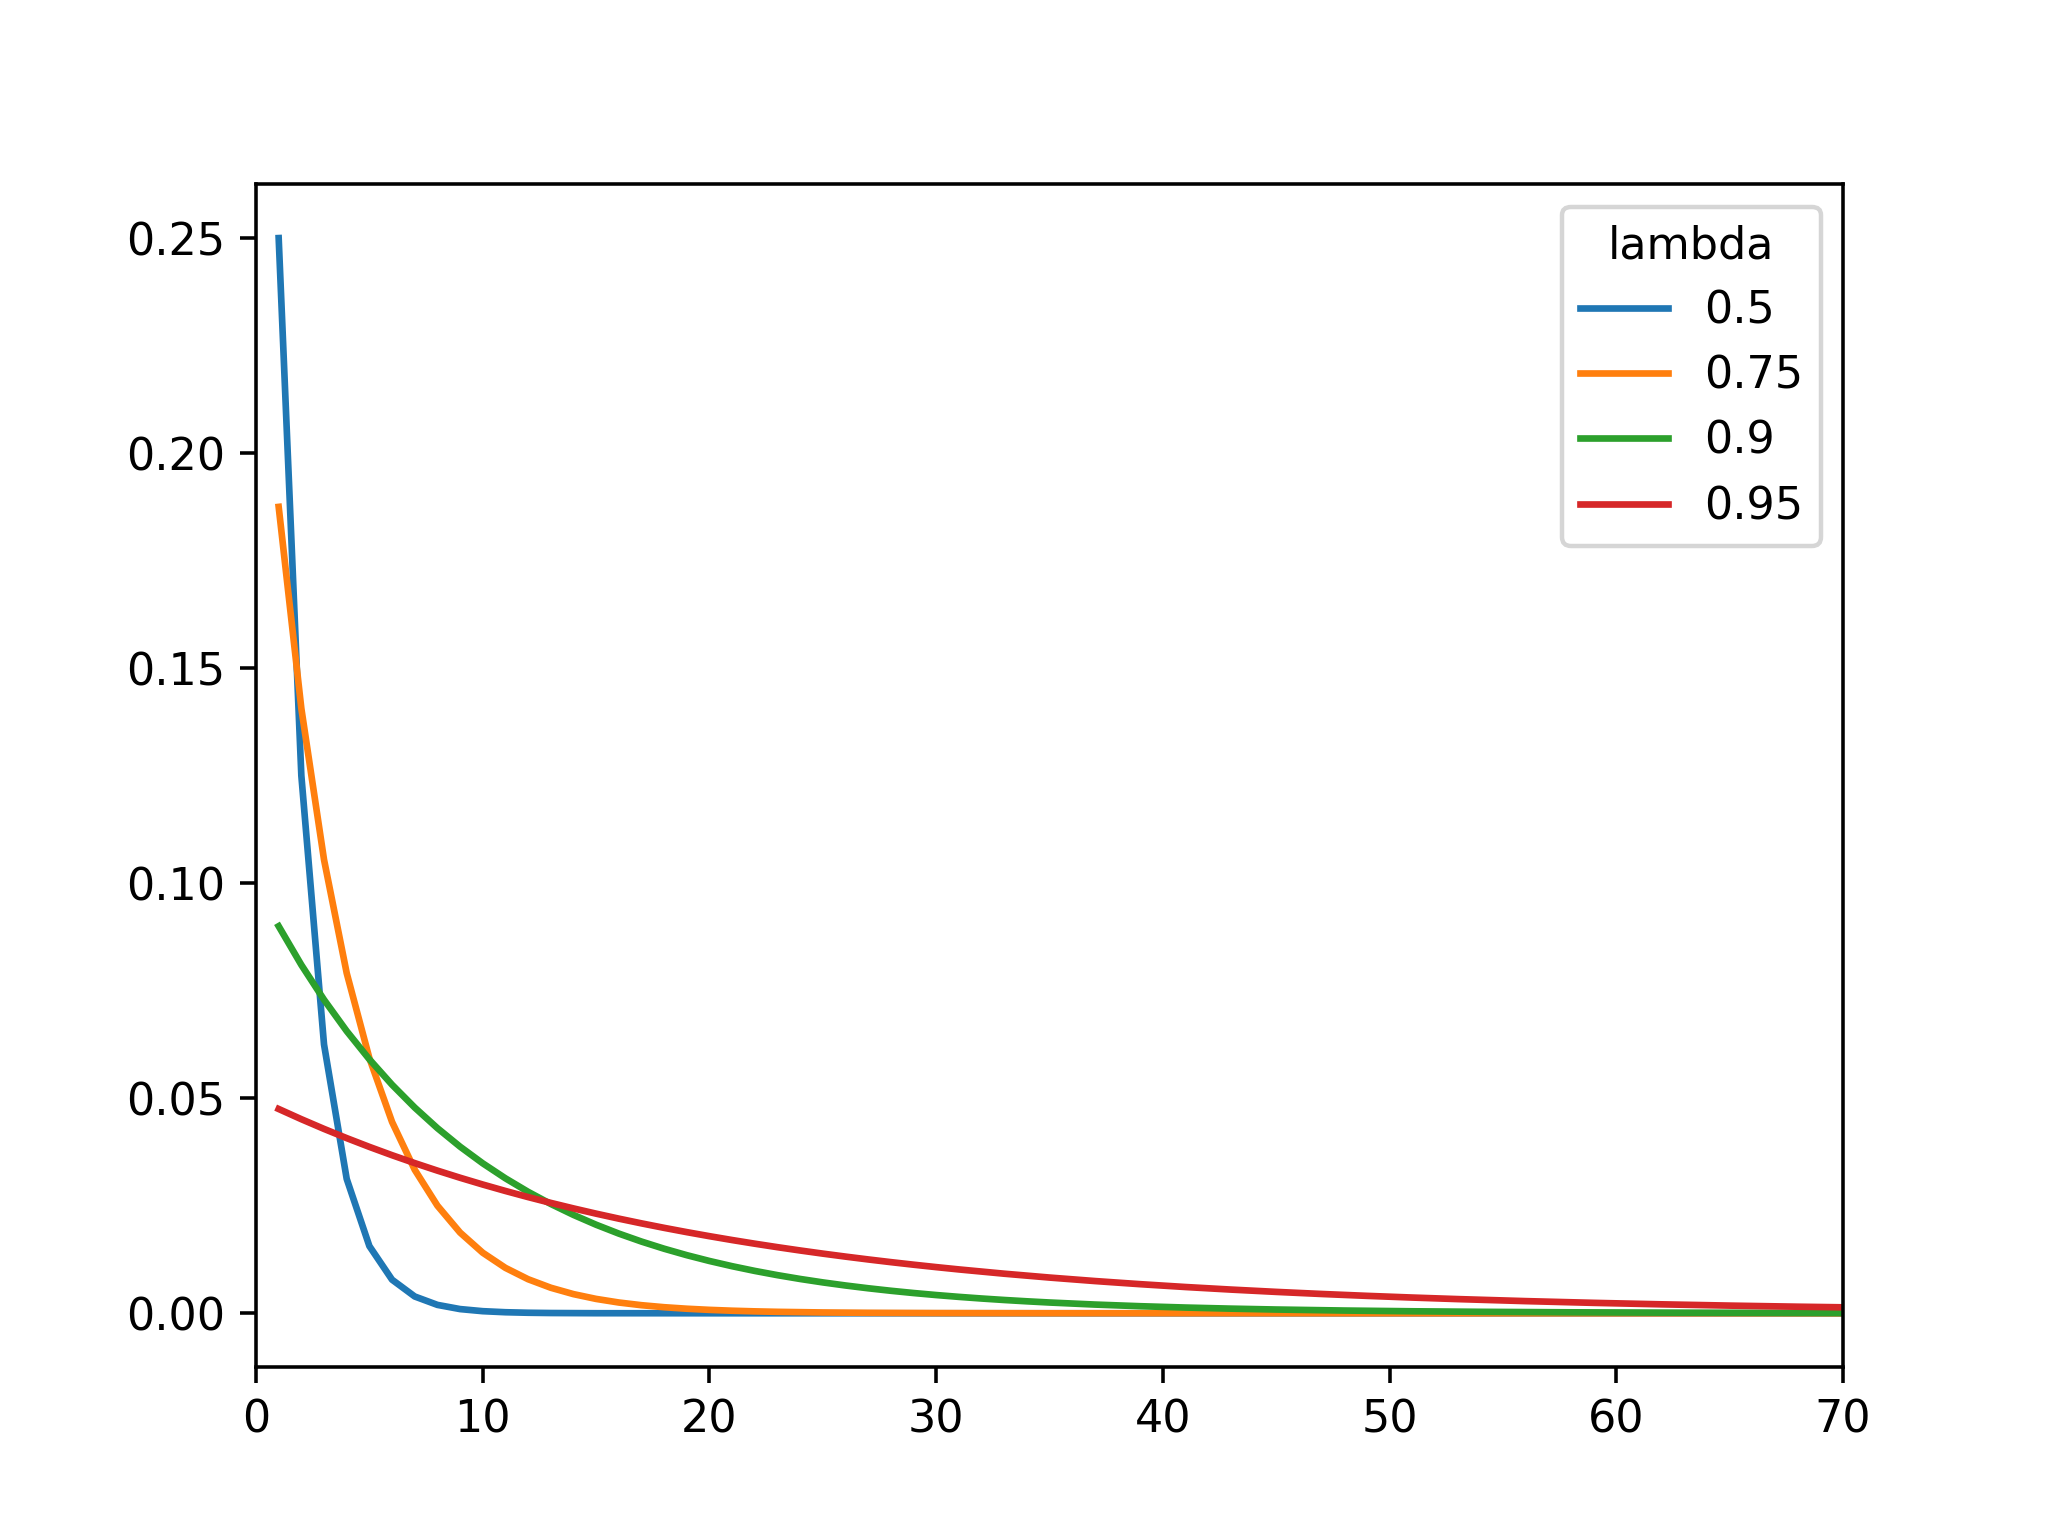
\includegraphics[width=0.75\textwidth]{images/lambda_return_weight.png}
    \caption{تاثیر پارامتر  $\lambda$ بر اهمیت پاداش‌های آینده. 
    محور افقی نماینده تعداد گام‌ها، و محور عمودی نماینده وزن این بازگشت متناظر با آن است.}\label{fig:td_lambda}
    
\end{figure}
\subsubsection{تی‌دی لامبدا رو به عقب}
در روش تی‌دی $\lambda$ با دید رو به عقب،
از مفهومی به نام آثار شایستگی \LTRfootnote{Eligibility Traces} استفاده می‌شود.
این مفهوم، نشان‌دهنده‌ی این است که هر عملی که در گذشته انجام شده و موجب تغییر ارزش عملی شده است،  به چه میزان روی این تغییر سهیم بوده‌است.

ابتدا به ازای هر حالت و عمل، یک متغیر آثار شایستگی $E(s, a)$
صفر تعیین می‌شود و سپس در هر گام، این متغیر به صورت زیر به روزرسانی می‌شود:
\begin{equation}\label{eq:eligibility_trace}
    E(s, a) = \gamma \times \lambda \times E(s, a) + 1(s = s_t, a = a_t)
\end{equation}
در واقع کل آثار شایستگی در لامبدا ضرب شده، و یکی به آثار شایستگی عمل و حالت فعلی اضافه می‌شود.
در این حالت، آثار شایستگی معادل با میزان نزدیکی زمانی هر حالت و عمل، به حالت و عمل فعلی است.

سپس ارزش عمل به صورت زیر به روزرسانی می‌شود:
\begin{equation}\label{eq:td_lambda_backward_q_function}
    Q(s, a) = Q(s, a) + \alpha \times \delta \times E(s, a)
\end{equation}
که در این رابطه، $\delta$
خطای تخمین است که به صورت زیر محاسبه می‌شود:
\begin{equation}\label{eq:td_lambda_backward_delta}
    \delta = R_{t+1} + \gamma \times (Q(s_{t+1}, a_{t+1}) - Q(s_t, a_t))
\end{equation}
می‌توان نشان داد که پس از انجام یک قسمت، به‌روز‌رسانی‌های انجام شده توسط این روش، معادل با به‌روز‌رسانی‌های انجام شده توسط تی‌دی $\lambda$ با دید رو به جلو است.

با ترکیب این روش و سیاست اپسیلون-حریصانه، می‌توان به یک روش یادگیری تقویتی کارا دست یافت که 
سارسا-لامبدا \LTRfootnote{SARSA($\lambda$)} نام دارد.
\section{استفاده از تقریب‌گر تابع}
با توجه به زیاد بودن تعداد حالت‌های ممکن در اکثر مسائل، یادگیری با روش‌های توضیح‌داده‌شده بسیار کند و حتی غیرمعقول می‌باشد.
از این رو، به جای نگه‌داری مقادیر \lr{Q} 
در یک جدول به ازای هر زوج حالت-عمل
 از تقریب‌گر‌های تابع\LTRfootnote{Function Approximators}
  برای تخمین این مقادیر استفاده می‌کنیم.

    از تقریب‌گر‌های تابع مختلفی می‌توان برای این کار استفاده کرد.
    از جمله‌ی این تقریب‌گر‌ها می‌توان به شبکه‌های عصبی، درخت‌های تصمیم، و توابع پایه‌ای مثل چندجمله‌ای‌ها اشاره کرد.

    در واقع ابتدا از حالت، برخی ویژگی‌های مهم را استخراج کرده، سپس از این ویژگی‌ها برای تخمین ارزش‌ها به کمک پارامتر‌هایی که قرار است یاد گرفته شوند استفاده می‌کنیم.
    رایج است که در روابط، به این پارامتر‌ها با 
    $\theta$ یا $w$
    اشاره شود.

\begin{figure}[H]
    \centering
    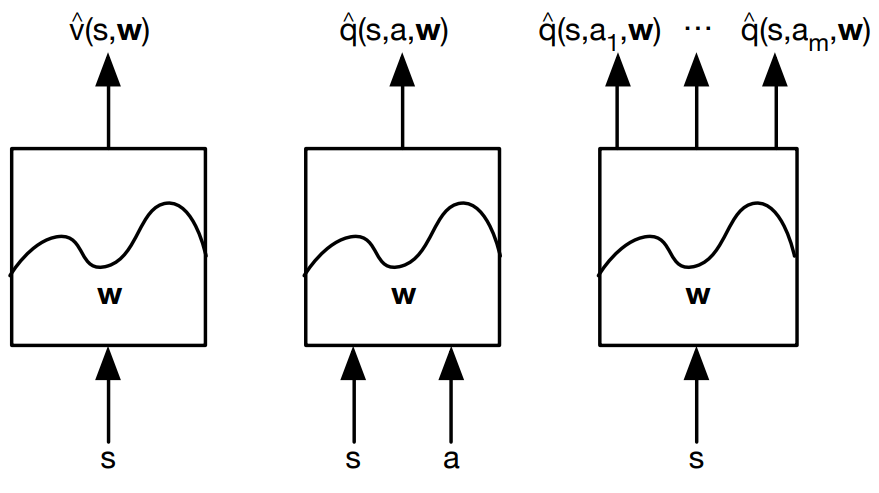
\includegraphics[width=0.75\textwidth]{images/function_approximators.png}
    \caption{روش‌های مختلف استفاده از تقریب‌گر تابع}\label{fig:func_approx}
\end{figure}
حال کافی‌ست که معادلات \ref{eq:td_zero_q_function}، \ref{eq:td_lambda_q_function}، و \ref{eq:td_lambda_backward_q_function} را به صورت تقریبی برای تقریب‌گر تابع بنویسیم،
و به‌جای به روزرسانی مقادیر \lr{Q}، پارامتر‌های تقریب‌گر تابع را به‌روز کنیم.
با توجه به نیاز به به‌روز‌رسانی، لازم است از تقریب‌گر‌های مشتق‌پذیر استفاده کنیم.
همانطور که در عکس \ref{fig:func_approx}
می‌توان دید، در حالتی که از تقریب‌گر‌های تابع برای پیش‌بینی مقادیر \lr{Q} استفاده می‌شود،
رایج است از عبارت 
$Q(s, a; \theta)$
یا $Q(s, a; w)$
برای نشان دادن این تقریب‌گر‌ها استفاده کرد.

\section{الگوریتم یادگیری \lr{Q} عمیق}
این الگوریتم، یکی از مستقیم‌ترین راه‌های استفاده از تقریب‌گر‌های توابع، برای ترکیب یادگیری عمیق و تقویتی است.
در این الگوریتم، هدف این است که مشابه با حالت سوم شکل \ref{fig:func_approx}،
پارامتر‌های یک شبکه عصبی را به‌گونه‌ای تنظیم کنیم که مقادیر ارزش-عمل را بتواند تخمین بزند.
از دستاورد‌های این الگوریتم، عملکرد در حد انسان در چندین بازی آتاری \LTRfootnote{Atari} است
که توسط تیم دیپ‌مایند \LTRfootnote{DeepMind}
در سال ۲۰۱۵ به‌وقوع پیوست.

شبکه‌های عصبی الهام گرفته از ساختار و عملکرد مغز انسان هستند که برای یادگیری از داده‌ها و تصمیم‌گیری‌های پیچیده استفاده می‌شوند.
 این شبکه‌ها از واحدهای پردازشی به نام پرسپترون‌ها تشکیل شده‌اند که در لایه‌های مختلف قرار گرفته‌اند و از طریق وزن‌هایی به هم متصل می‌شوند.
 
 یادگیری در شبکه‌های عصبی اغلب از طریق فرایندی به نام نزول گرادیان انجام می‌گیرد که در آن وزن‌های شبکه به صورت تکراری تنظیم می‌شوند تا خطا بین پیش‌بینی‌های شبکه و داده‌های واقعی به حداقل برسد. این فرایند شامل محاسبه گرادیان یا شیب تابع خطا نسبت به وزن‌ها و به‌روزرسانی وزن‌ها در جهت مخالف گرادیان برای کاهش خطا است.
% formula for gradient descent
\begin{equation}\label{eq:gradient_descent}
    \theta_{t+1} = \theta_t - \alpha \nabla J(\theta_t)
\end{equation}
در این فرمول، $\theta$
پارامتر‌های شبکه،
\lr{$\alpha$}
نرخ یادگیری،
\lr{$J$}
تابع خطا، و
\lr{$\nabla J$}
گرادیان تابع خطا نسبت به پارامتر‌ها هستند.

برای اینکه یادگیری شبکه عصبی با ثبات بالاتری رخ دهد، این الگوریتم از دو تکنیک 
\textbf{بازیابی تجربه}
و
\textbf{استفاده از شبکه هدف}
بهره می‌برد.
\subsection{بازیابی تجربه}
برای رفع مشکلات داده‌های همبسته و توزیع‌های غیر ایستا در یادگیری آنلاین، \lr{DQN} از یک مکانیزم بازیابی تجربه استفاده می‌کند. این شامل ذخیره تجربیات عامل در هر گام زمانی در یک بافر بازیابی و سپس نمونه‌برداری تصادفی ریزدسته‌ها \LTRfootnote{Mini-batches}
 از این بافر برای آموزش شبکه است. این رویکرد به شکستن همبستگی بین نمونه‌های پیاپی کمک می‌کند و فرآیند یادگیری را پایدار می‌سازد.
\subsection{استفاده از شبکه هدف}
\lr{DQN} یک شبکه دوم به نام شبکه هدف را برای استقرار بیشتر آموزش معرفی می‌کند. شبکه هدف یک کپی از شبکه \lr{Q} است، اما وزن‌های آن کمتر به‌روز می‌شوند. این جداسازی نوسان ارزش‌های هدف در به‌روزرسانی یادگیری \lr{Q} را کاهش می‌دهد و خطر حلقه‌های بازخورد خودتقویتی را کاهش می‌دهد.
\subsection{فرآیند یادگیری}
در ابتدا وزن‌های شبکه ارزش-عمل را به صورت تصادفی تنظیم می‌کنیم و آن را $\theta$ می‌نامیم.
 شبکه هدف را با وزن‌های یکسان مقداردهی می‌کنیم و آن را $\theta^-$ می‌نامیم.
و بافر بازیابی را
به طول $N$ که یک ابرپارامتر است، مقداردهی می‌کنیم.

سپس در هر حالت، پاداش‌های خروجی شبکه اصلی را می‌گیریم و به صورت اپسیلون-حریصانه عمل را انتخاب می‌کنیم؛
یعنی به احتمال $\epsilon$ رفتار تصادفی داریم، 
و با احتمال $1-\epsilon$
رفتار با بالاترین ارزش-عمل پیش‌بینی شده را برمیداریم، یعنی: $a_t = \underset{a}{\mathrm{argmax}} Q(s_t, a; \theta)$.
ترکیب چهارتایی حالت قبل عمل، عمل انتخاب شده، پاداش دریافتی، و حالت بعد عمل $(s_t,a_t,r_t,s_{t+1})$
را به بافر اضافه می‌کنیم.
یک گروه با اندازه مشخص را با نمونه‌برداری تصادفی از بافر انتخاب می‌کنیم، و به صورت زیر یادگیری را انجام می‌دهیم:
\begin{equation}\label{dqn_label}
    y_j = \begin{cases}
        r_j & \text{اگر $s_{j+1}$ حالت پایانی قسمت باشد} \\
        r_j + \gamma \times \max_{a'} Q(s_{j+1}, a'; \theta^-) & \text{در غیر این صورت}
    \end{cases}
\end{equation}
در این معادله $y_j$ تخمینی از میزان پاداش دریافتی واقعی است، که مشابه با روش‌های \lr{TD}، از ترکیب پاداش دریافتی و ارزش-عمل بعدی به دست می‌آید.
بنابرین می‌توان از این مقدار، مشابه با برچسب در یادگیری نظارت‌شده، برای آموزش شبکه استفاده کرد.
میزان خطای شبکه به صورت زیر تعریف می‌شود:
\begin{equation}\label{dqn_loss}
    L(\theta) = \mathbb{E}[(y_j - Q(s_j, a_j; \theta))^2]
\end{equation}
که با استفاده از این خطا، می‌توان گرادیان تابع خطا نسبت به وزن‌های شبکه را به دست آورد و
با استفاده از این گرادیان، می‌توان وزن‌های شبکه را به‌روز کرد:
\begin{equation}\label{dqn_update}
    \theta_{t+1} = \theta_t - \alpha \nabla_\theta L(\theta)
\end{equation}
در نهایت کافی‌ست به صورت تناوبی و هر چند گام یک بار وزن‌های شبکه هدف را برابر با کپی وزن‌های شبکه اصلی قرار دهیم. با تکرار این مراحل، به شبکه عصبیی دست می‌یابیم که قدرت پیش‌بینی ارزش‌های عمل را دارد.


حال می‌توان اهمیت دو تکنیک گفته شده را بهتر فهمید: در صورت عدم استفاده از شبکه هدف، باید همزمان از شبکه اصلی برای پیش‌بینی آینده (در فرمول \ref{dqn_label}) و انتخاب عمل استفاده کنیم، که می‌تواند به مشکلاتی مانند نوسانات در آموزش و حلقه‌های بازخورد خودتقویتی منجر شود.
همچنین در صورت عدم استفاده از بافر تجربه، باید صرفا از تجارب اخیر خود استفاده کنیم، که در این صورت هبستگی بین نمونه‌ها و توزیع‌های غیر ایستا می‌تواند مشکل‌ساز شود.
\section{الگوریتم بهبود گرادیان سیاست معین عمیق}
الگوریتم بهبود گرادیان سیاست معین عمیق \LTRfootnote{Deep Deterministic Policy Gradient} یا به اختصار \lr{DDPG}، یک الگوریتم یادگیری تقویتی است که برای حل مسائل پیوسته و فضای عمل پیوسته طراحی شده است.
همانطور که در بخش‌های قبل دیدیم، برای انتخاب عمل معمولا از سیاست اپسیلون-حریصانه استفاده می‌شود، اما این روش برای فضای عمل پیوسته مناسب نیست، چرا که به‌دست‌آوردن بیشینه در فضای پیوسته به مراتب دشوار‌تر از حالت گسسته است.
این الگوریتم از نوع یادگیری خارج از سیاست است؛ به این معنا که عامل با دنبال کردن سیاستی که سیاست انتخابی خود نیست به بهبود عملکرد خود می‌پردازد.

\lr{DDPG}
از دو شبکه عصبی استفاده می‌کند: یک شبکه برای تخمین ارزش عمل که به آن نقاد می‌گوییم، و یک شبکه برای تخمین سیاست و انتخاب عمل که به آن بازیگر می‌گوییم.
شبکه نقاد مشابه با شبکه
 \lr{Q}
  در 
  \lr{DQN}
   است، با این تفاوت که حالت و عمل را ورودی گرفته و ارزش عمل را خروجی می‌دهد.
 و شبکه سیاست یک شبکه عصبی است که خروجی آن عمل است.
 این الگوریتم مشابه با \lr{DQN}
 از بافر تجربه برای ذخیره تجربیات عامل، و از شبکه‌های هدف برای هر دو شبکه نقاد و بازیگر استفاده می‌کند.
 البته در این الگوریتم، به‌جای کپی وزن‌های شبکه به شبکه هدف، از میانگین وزن‌دار استفاده می‌شود تا به روز‌رسانی آرام‌تر انجام شود و ثبات بیشتری داشته باشد.
 \begin{figure}[H]
    \centering
    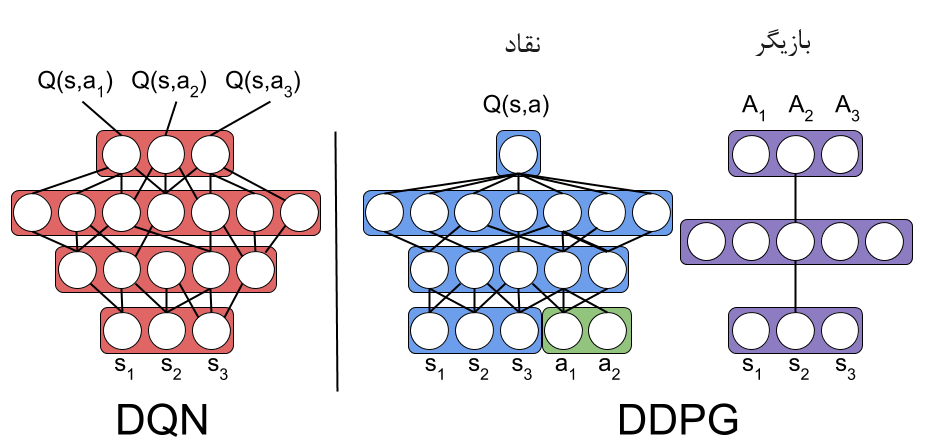
\includegraphics[width=0.85\textwidth]{images/actor_critic.png}
    \caption{شبکه‌های عصبی بازیگر و نقاد در الگوریتم \lr{DDPG} و مقایسه با \lr{DQN}}\label{fig:actor_critic}
\end{figure}
رایج است که شبکه ارزش عمل را با $Q(s, a; \phi)$ و شبکه سیاست را با $\mu(s; \theta)$ نشان دهیم.
فرآیند یادگیری این الگوریتم به صورت زیر است:
\begin{enumerate}
    \item ابتدا وزن‌های شبکه‌های نقاد و بازیگر را به صورت تصادفی مقداردهی می‌کنیم و آن‌ها را به ترتیب $\phi$ و $\theta$ می‌نامیم.
    \item بافر تجربه را به طول $N$ مقداردهی می‌کنیم.
    \item در هر گام زمانی، حالت را به شبکه بازیگر می‌دهیم و عملی که این شبکه پیشنهاد می‌دهد را انجام می‌دهیم.
    \item پاداش دریافتی و حالت بعد عمل را به بافر تجربه اضافه می‌کنیم.
    \item یک ریزدسته از بافر تجربه را انتخاب کرده و با استفاده از فرمول زیر، مقدار واقعی ارزش حالت را (طبق الگوریتم \lr{TD}) محاسبه می‌کنیم:
    \begin{equation}\label{ddpg_label}
        y_j = \begin{cases}
            r_j & \text{اگر $s_{j+1}$ حالت پایانی قسمت باشد} \\
            r_j + \gamma \times Q(s_{j+1}, \mu(s_{j+1}; \theta^-); \phi^-) & \text{در غیر این صورت}
        \end{cases}
    \end{equation}
    \item خطای شبکه نقاد را به صورت زیر محاسبه می‌کنیم:
    \begin{equation}\label{ddpg_critic_loss}
        L(\phi) = \mathbb{E}[(y_j - Q(s_j, a_j; \phi))^2]
    \end{equation}
    و وزن‌های شبکه نقاد را به‌روز می‌کنیم:
    \begin{equation}\label{ddpg_critic_update}
        \phi_{t+1} = \phi_t - \alpha \nabla_\phi L(\phi)
    \end{equation}
    \item خطای شبکه بازیگر را به صورت زیر محاسبه می‌کنیم:
    \begin{equation}\label{ddpg_actor_loss}
        L(\theta) = -\mathbb{E}[Q(s, \mu(s; \theta); \phi)]
    \end{equation}
    و وزن‌های شبکه بازیگر را به‌روز می‌کنیم:
    \begin{equation}\label{ddpg_actor_update}
        \theta_{t+1} = \theta_t + \alpha \nabla_\theta L(\theta)
    \end{equation}
    \item در نهایت هر چند گام یک بار، وزن‌های شبکه‌های هدف را به‌روز می‌کنیم:
    \begin{equation}\label{ddpg_target_actor_update}
        \theta^-_{t+1} = \tau \theta_t + (1-\tau) \theta^-_t
    \end{equation}
    \begin{equation}\label{ddpg_target_critic_update}
        \phi^-_{t+1} = \tau \phi_t + (1-\tau) \phi^-_t
    \end{equation}
\end{enumerate}
همانطور که مشاهده‌شد، این الگوریتم تعداد زیادی پارامتر دارد که باید به‌درستی تنظیم شوند تا به عملکرد بهینه برسد.
از جمله این پارامتر‌ها می‌توان به نرخ یادگیری ($\alpha$ که می‌تواند برای شبکه‌های نقاد و بازیگر متفاوت باشد)،
، نرخ تخفیف ($\gamma$)،
فرکانس به‌روزرسانی شبکه‌ها (هر چند گام یک بار ریزدسته انتخاب می‌کنیم و مراحل ۵ تا ۸ را طی می‌کنیم)،
فرکانس به‌روزرسانی وزن‌های هدف (هر چند گام یک بار وزن‌های شبکه‌های هدف را به‌روزرسانی می‌کنیم)
 ، اندازه ریزدسته، طول بافر تجربه، و ضریب به‌روزرسانی شبکه‌های هدف $\tau$
  اشاره کرد.
\section{جمع‌بندی}

% پیش‌بینی داده‌های سری زمانی از زمان گذشته مورد توجه محققین و متخصصین بوده است. در نتیجه در گذر زمان روش‌های متنوعی برای این موضوع پیشنهاد شده‌اند.
% .آمار و احتمالات از علوم بسیار قدیمی بشریت محسوب میشود یکی از روش‌های قدیمی برای پیش‌بینی داده‌های سری زمانی میباشد در کنار این روش، روش‌های مهندسی نیز در دهه‌های گذشته استفاده شده‌اند.
% در این فصل برای ارائه‌ی یک دید جامع و مناسب در مورد پیش‌بینی مصرف انرژی ساختمان‌ها در مورد هر دو روش گفته شده صحبت میکنیم و در نهایت در مورد روش‌های هوش‌مصنوعی توضیحاتی را ارائه میکنیم.


% \section{روش آماری}

% مدل‌های رگرسیون آماری صرفا مصرف انرژی یا شاخص انرژی را با متغیرهای تأثیرگذار مرتبط می‌کنند. این مدل‌های تجربی از داده‌های عملکرد تاریخی ایجاد شده‌اند، به این معنی که قبل از آموزش مدل‌ها، باید داده‌های تاریخی کافی را جمع‌آوری کنیم. تحقیقات زیادی بر روی مدل های رگرسیون در مورد مسائل زیر انجام شده است. اولین مورد پیش بینی مصرف انرژی بر روی متغیرهای ساده شده مانند یک یا چند پارامتر آب و هوا است. مورد دوم پیش بینی برخی از شاخص انرژی مفید است. مورد سوم، تخمین پارامترهای مهم مصرف انرژی، مانند ضریب تلفات حرارتی کل، ظرفیت حرارتی کل و ضریب افزایش است که در تحلیل رفتار حرارتی ساختمان یا سیستم‌های سطح فرعی مفید هستند.
% \\
% در برخی از مدل‌های مهندسی ساده‌شده، از رگرسیون برای ارتباط مصرف انرژی با متغیرهای آب و هوایی برای به دست آوردن امضای انرژی استفاده می‌شود \cite{pfafferott2005thermal,bauer1998simplified}. بائر\LTRfootnote{Bauer} و اسکارتزینی\LTRfootnote{Scartezzini} \cite{bauer1998simplified} یک روش رگرسیون را برای انجام محاسبات گرمایش و سرمایش به طور همزمان با پرداختن به سودهای داخلی و همچنین خورشیدی پیشنهاد کردند. دار\LTRfootnote{Dhar} و همکاران \cite{dhar1998modeling,dhar1999fourier} بار گرمایش و سرمایش را در ساختمان‌های تجاری با دمای حباب خشک در فضای باز به عنوان تنها متغیر آب و هوا مدل‌سازی کرد. یک مدل سری فوریه مبتنی بر دما برای نشان دادن وابستگی غیرخطی بارهای گرمایش و سرمایش به زمان و دما پیشنهاد شد. اگر داده‌های رطوبت و خورشید نیز در دسترس باشد، آنها استفاده از مدل سری فوریه تعمیم‌یافته را پیشنهاد کردند زیرا ارتباط مهندسی بیشتر و توانایی پیش‌بینی بالاتری دارد. همچنین با در نظر گرفتن دمای حباب خشک به عنوان متغیر واحد برای توسعه مدل، لی\LTRfootnote{Lei} و هو\LTRfootnote{Hu} \cite{lei2009baseline} مدل‌های رگرسیونی را برای پیش‌بینی صرفه‌جویی در انرژی از پروژه‌های مقاوم‌سازی ساختمان‌های اداری در یک منطقه تابستانی گرم و زمستانی سرد ارزیابی کردند. آنها نشان دادند که یک مدل خطی تک متغیری برای مدلسازی مصرف انرژی در شرایط آب و هوایی گرم و سرد کافی و کاربردی است. ما\LTRfootnote{Ma} و همکاران\cite{ma2010study} روش‌های رگرسیون خطی چندگانه و خود رگرسیون را برای پیش‌بینی مصرف انرژی ماهانه برای ساختمان‌های عمومی در مقیاس بزرگ ادغام کرد. در کار چو\LTRfootnote{Cho} و همکاران.\cite{cho2004effect}، مدل رگرسیون در اندازه‌گیری‌های 1 روزه، 1 هفته‌ای و 3 ماهه ایجاد شد که منجر به خطای پیش‌بینی در مصرف انرژی سالانه 100\%، 30\%، 6\% شد. این نتایج نشان می دهد که طول دوره اندازه گیری به شدت بر مدل های رگرسیون وابسته به دما تأثیر می گذارد.
% \\
% در مورد پیش‌بینی شاخص انرژی، لام\LTRfootnote{Lam} و همکاران.\cite{lam2010principal} از تجزیه و تحلیل اجزای اصلی \LTRfootnote{PCA} برای ایجاد یک شاخص آب و هوایی زد\LTRfootnote{Z} با توجه به تابش خورشیدی جهانی، دمای حباب خشک و مرطوب استفاده کرد. آنها دریافتند که زد همان روندی را دارد که بار سرمایشی شبیه سازی شده، تهویه مطبوع و مصرف انرژی ساختمان را نشان می دهد. این روند از تحلیل همبستگی با تحلیل رگرسیون خطی به دست آمد. این مدل بر اساس داده های 1979 تا 2007 توسعه یافته است.

% \section{روش مهندسی}


% روش های مهندسی از اصول فیزیکی برای محاسبه دینامیک حرارتی و رفتار انرژی در کل سطح ساختمان یا برای اجزای سطح فرعی استفاده می کنند. آنها در طول پنجاه سال گذشته به اندازه کافی توسعه یافته اند. این روش ها را می توان به طور تقریبی به دو دسته روش جامع تفصیلی و روش ساده شده طبقه بندی کرد. روش‌های جامع از توابع فیزیکی بسیار دقیق یا دینامیک حرارتی برای محاسبه دقیق، گام به گام، مصرف انرژی برای همه اجزای ساختمان با اطلاعات ساختمان و محیط‌زیست، مانند شرایط اقلیمی خارجی، ساخت و ساز ساختمان، بهره‌برداری، برنامه نرخ بهره‌برداری استفاده می‌کنند. و تجهیزات گرمایش و تهویه هوا به عنوان ورودی. در این مقاله، ما بر دیدگاه جهانی مدل‌ها و برنامه‌ها تمرکز می‌کنیم، در حالی که جزئیات این فرآیندهای محاسباتی بسیار فراتر از هدف این بررسی است. خوانندگان ممکن است برای جزئیات محاسبه به \cite{clarke2001energy} مراجعه کنند. برای سیستم های گرمایش و تهویه هوا، به طور خاص، محاسبه دقیق انرژی در \cite{mcquiston2004heating} معرفی شده است. سازمان بین المللی استاندارد سازی، استانداردی برای محاسبه مصرف انرژی برای گرمایش و سرمایش فضا برای یک ساختمان و اجزای آن ایجاد کرده است. صدها ابزار نرم افزاری برای ارزیابی کارایی انرژی، انرژی های تجدیدپذیر و پایداری در ساختمان ها توسعه یافته اند. برخی از آنها به طور گسترده برای توسعه استانداردهای انرژی ساختمان و تجزیه و تحلیل مصرف انرژی و اقدامات حفاظتی ساختمان ها مورد استفاده قرار گرفته اند. این ابزارها در مقاله های \cite{CRAWLEY2008661,al2001computer} بررسی شده اند. وزارت انرژی ایالات متحده فهرستی از تقریبا تمام ابزارهای شبیه سازی را که دائما به روز می شود، نگهداری می کند.
% \\
% اگرچه این ابزارهای شبیه سازی دقیق موثر و دقیق هستند، اما در عمل مشکلاتی وجود دارد. از آنجایی که این ابزارها مبتنی بر اصول فیزیکی هستند، برای رسیدن به یک شبیه‌سازی دقیق، به جزئیات ساختمان و پارامترهای محیطی به عنوان داده‌های ورودی نیاز دارند. از یک طرف، این پارامترها برای بسیاری از سازمان ها در دسترس نیستند، به عنوان مثال، اطلاعات مربوط به هر اتاق در یک ساختمان بزرگ همیشه دشوار است. این عدم وجود ورودی های دقیق منجر به شبیه سازی با دقت پایین می شود. از سوی دیگر، به کارگیری این ابزارها معمولا نیازمند کار کارشناسی خسته کننده است که انجام آن را دشوار و هزینه را کم می کند. به این دلایل برخی از محققان مدل های ساده تری را برای ارائه جایگزین هایی برای کاربردهای خاص پیشنهاد کرده اند.
% \\
% الحمود\LTRfootnote{Al-Homoud} \cite{al2001computer} دو روش ساده شده را بررسی کرد. یکی روش درجه روز است که در آن تنها یک شاخص یعنی درجه روز تحلیل می شود. این روش حالت پایدار برای تخمین مصرف انرژی ساختمان های کوچک که در آن انرژی مبتنی بر پوشش غالب است، مناسب است. یکی دیگر از سطل، همچنین به عنوان روش فرکانس دما شناخته می شود، که می تواند برای مدل سازی ساختمان های بزرگ استفاده شود که در آن بارهای تولید شده داخلی غالب هستند یا بارها به طور خطی به اختلاف دمای بیرون و داخل خانه وابسته نیستند.
% \\
% شرایط آب و هوایی عوامل مهمی برای تعیین میزان مصرف انرژی ساختمان هستند. اینها اشکال مختلفی مانند دما، رطوبت، تابش خورشیدی، سرعت باد دارند و در طول زمان تغییر می کنند. مطالعات خاصی برای ساده کردن شرایط آب و هوایی در محاسبات انرژی ساختمان انجام شده است.






% \section{روش هوش مصنوعی}

% روش های هوش مصنوعی در سال‌های اخیر رشد در زمینه‌ی پیش‌بینی مصرف انرژی ساختمان‌ها رشد بسیار زیادی داشته اند. به علت سهولت بهتر و دقت بالای این روش در سال‌های اخیر روش غالب در پیش‌بینی مصرف انرژی ساختمان‌ها این نوع روش‌ها بوده‌اند. 
% در این بخش دو زیر بخش مهم از روش‌های هوش مصنوعی مورد بررسی قرار گرفته‌اند. 

% \subsection[شبکه‌های عصبی]{شبکه‌های عصبی\protect\LTRfootnote{Neural Networks}}

% شبکه های عصبی مصنوعی پرکاربردترین مدل های هوش مصنوعی در کاربرد پیش بینی انرژی ساختمان هستند. این نوع مدل در حل مسائل غیر خطی خوب است و یک رویکرد موثر برای این کاربرد پیچیده است. در بیست سال گذشته، محققان از شبکه‌های عصبی مصنوعی برای تجزیه و تحلیل انواع مختلف مصرف انرژی ساختمان در شرایط مختلف، مانند بار گرمایش/سرمایش، مصرف برق، عملکرد و بهینه‌سازی اجزای سطح زیرین، تخمین پارامترهای مصرف استفاده کرده‌اند. در این بخش، مطالعات قبلی را مرور می کنیم و با توجه به کاربردهایی که به آن پرداخته شده، آنها را در گروه هایی قرار می دهیم. علاوه بر این، بهینه سازی مدل، مانند پیش فرآیند داده های ورودی و مقایسه بین شبکه های عصبی مصنوعی و سایر مدل ها، در پایان برجسته شده است. در سال 2006، کالوگیرو\LTRfootnote{Kalogirou} \cite{kalogirou1997building} مروری کوتاه بر شبکه‌های عصبی مصنوعی در کاربردهای انرژی در ساختمان‌ها، از جمله سیستم‌های گرمایش آب خورشیدی، تابش خورشیدی، سرعت باد، توزیع جریان هوا در داخل اتاق، پیش‌بینی مصرف انرژی، دمای هوای داخل ساختمان و سیستم گرمایش و تهویه هوا انجام داد.
% کالوگیرو و همکاران \cite{kalogirou2006artificial} از شبکه های عصبی پس انتشار\LTRfootnote{back propagation neural networks} برای پیش بینی بار گرمایش مورد نیاز ساختمان ها استفاده کرد. این مدل بر روی داده های مصرف 225 ساختمان آموزش داده شد که تا حد زیادی از فضاهای کوچک تا اتاق های بزرگ متفاوت است. اولوفسون و همکاران \cite{olofsson1998method} تقاضای گرمایش سالانه تعدادی از ساختمان‌های کوچک خانواده‌ای در شمال سوئد را پیش‌بینی کرد. بعدا، اولوفسون\LTRfootnote{Olofsson} و اندرسون\LTRfootnote{Anderson}\cite{olofsson2001long} یک شبکه عصبی ایجاد کردند که تقاضای انرژی بلندمدت (تقاضای گرمایش سالانه) را بر اساس داده‌های اندازه‌گیری شده کوتاه‌مدت (معمولا 2 تا 5 هفته) با نرخ پیش‌بینی بالا برای ساختمان‌های تک خانواده پیش‌بینی می‌کند.


% \subsection[ماشین بردار پشتیبان]{ماشین بردار پشتیبان\protect\LTRfootnote{Support Vector Machine(SVM)}}

% ماشین‌های بردار پشتیبان به طور فزاینده ای در تحقیقات و صنعت مورد استفاده قرار می گیرند. آنها مدل های بسیار موثری در حل مسائل غیر خطی حتی با مقادیر کم داده های آموزشی هستند. مطالعات بسیاری از این مدل ها در مورد تجزیه و تحلیل انرژی ساختمان در پنج سال گذشته انجام شده است.
% دونگ\LTRfootnote{Dong} و همکاران \cite{dong2005applying} برای اولین بار از ماشین بردار پشتیبان برای پیش بینی مصرف برق ماهانه چهار ساختمان در منطقه گرمسیری استفاده کرد. داده های سه ساله آموزش داده شد و مدل مشتق شده برای پیش بینی سودمندی مالک در آن سال بر روی داده های یک ساله اعمال شد. نتایج نشان دهنده عملکرد خوب ماشین‌های بردار پشتیبان در این مشکل بود.
% \\
% لای\LTRfootnote{Lai} و همکاران\cite{lai2008vapnik} این مدل را بر مصرف برق یکساله یک ساختمان اعمال کرد. متغیرها شامل تغییرات آب و هوایی است. در آزمایشات آنها، این مدل از عملکرد یک سال استخراج شد و سپس بر روی رفتار سه ماهه آزمایش شد. آنها همچنین مدل را بر روی هر مجموعه داده روزانه آزمایش کردند تا پایداری این رویکرد را در دوره‌های کوتاه تأیید کنند. علاوه بر این، آنها اغتشاش را به صورت دستی به بخش خاصی از عملکرد تاریخی اضافه کردند و از این مدل برای تشخیص اغتشاش با بررسی تغییر وزن های کمک کننده استفاده کردند.
% \\
% لیانگ\LTRfootnote{Liang} و دو\LTRfootnote{Du} \cite{liang2007model} یک روش تشخیص عیب مقرون به صرفه را برای سیستم های گرمایش و تهویه هوا با ترکیب مدل فیزیکی و یک ماشین بردار پشتیبان ارائه کردند. با استفاده از طبقه‌بندی کننده چهار لایه ماشین بردار پشتیبان، می‌توان وضعیت عادی و سه خطای احتمالی را با تعداد کمی از نمونه‌های آموزشی به سرعت و با دقت تشخیص داد.

% \section{خلاصه}

% با توجه به توصیف و تحلیل فوق، بدیهی است که برای ارزیابی سیستم انرژی ساختمان، از سطح زیرسیستم تا سطح ساختمان و حتی سطح منطقه ای یا ملی، محاسبات زیادی مورد نیاز است. 
% هر مدل در موارد خاصی از کاربردها مزایای خاص خود را دارد. مدل مهندسی تغییرات زیادی را نشان می دهد. ملاحظات زیادی می تواند در توسعه این مدل دخیل باشد. می تواند یک مدل
%  بسیار پیچیده و جامع باشد که برای محاسبات دقیق قابل استفاده است. در مقابل، با اتخاذ برخی استراتژی‌های ساده‌کننده، می‌توان آن را به یک مدل سبک تبدیل کرد و با حفظ دقت، توسعه
%  آن آسان است. یک اشکال رایج پذیرفته شده این مدل مهندسی دقیق این است که به دلیل پیچیدگی زیاد و کمبود اطلاعات ورودی، اجرای آن در عمل دشوار است. توسعه مدل آماری نسبتا 
% آسان است اما اشکالات آن نیز مشهود است که عبارتند از عدم دقت و عدم انعطاف پذیری. شبکه‌های عصبی مصنوعی و ماشین‌های بردار پشتیبان در حل مسائل غیر خطی خوب هستند و آنها را
%  برای پیش بینی انرژی ساختمان کاربردی می کند. تا زمانی که انتخاب مدل و تنظیم پارامترها به خوبی انجام شود، آنها می توانند پیش بینی بسیار دقیقی ارائه دهند.
%  ماشین‌های بردار پشتیبان حتی در بسیاری از موارد عملکرد بهتری نسبت به شبکه‌های عصبی مصنوعی نشان می دهند\cite{li2010prediction}. معایب این دو نوع مدل این است که به داده های عملکرد تاریخی
%   کافی نیاز دارند و بسیار پیچیده هستند.
%   تجزیه و تحلیل مقایسه ای این مدل های رایج در جدول 1 خلاصه شده است.
% \begin{table}
%     \caption[خلاصه‌ی کلی از متد‌های پیش‌بینی و ویژگی های هریک]{خلاصه‌ی کلی از متد‌های پیش‌بینی و ویژگی های هریک}
%     \begin{tabular}{ |p{2cm}|p{2cm}|p{2cm}|p{2cm}|p{2cm}|p{2cm}|  }
%         \hline
%         متد & پیچیدگی مدل  &سادگی استفاده&سرعت اجرا& نیازهای ورودی& دقت\\
%         \hline
%         مهندسی دقیق& نسبتا بالا& غیرساده& کم& با جزئیات& نسبتا بالا\\
%         \hline
%         مهندسی ساده‌سازی شده& بالا& ساده& بالا& ساده‌سازی شده& بالا\\
%         \hline
%         آماری& معمولی& ساده& نسبتا بالا& داده‌های تاریخی& معمولی\\
%         \hline
%         شبکه‌های عصبی مصنوعی& بالا& غیرساده& بالا& داده‌های تاریخی& بالا\\
%         \hline
%         ماشین بردار پشتیبان& نسبتا بالا& غیرساده& کم& داده‌های تاریخی& نسبتا بالا\\
%         \hline
%         \end{tabular}
% \end{table}